\documentclass[12pt,letterpaper]{article}
\usepackage{graphicx}
\usepackage{ifpdf}

\usepackage{multicol}
\usepackage{tikz}

\usepackage{amssymb}
\usepackage{amsmath}

\usepackage{caption}
\usepackage{subcaption}

\usepackage{hyperref}
% \usepackage{cite}

%\usepackage[backend=bibtex]{biblatex}
%\bibliography{bibliografia} 

\hypersetup{
    colorlinks=true,
    linkcolor=black,
    citecolor = black,
%     filecolor=magenta,      
    urlcolor=black,
%     pdftitle={GSP Toolbox Manual},
    bookmarks=true
%     pdfpagemode=FullScreen,
}

\usepackage[spanish]{babel}

\usepackage{fancyhdr}
 
\pagestyle{fancy}
\fancyhf{}
\rhead{Isaac Ayala Lozano\\194520009 \hspace{2 em}   \textbf{\#2}}
\lhead{}
\fancyfoot[R]{\thepage}

\begin{document}
\pagenumbering{gobble}
\section*{Péndulo Simple}

Se presentan los resultados de la simulación para el 
péndulo simple evaluado con fricción y sin fricción.
Las condiciones de simulación se muestran en la
tabla \ref{table: initial conditions}

\begin{table}[h]
\begin{center}
\centering
\begin{tabular}{cccc}
\hline
Tiempo inicial ($t_0$) & 0  & Posición angular inicial ($\theta_0$) & $\frac{\pi}{18}$ \\
%\hline
Tiempo final ($t_f$) & 10 & Velocidad angular inicial ($\dot{\theta}_0$)& $1$\\
Masa ($m$) & 1 & Longitud ($l$) & 1\\
Constante de gravedad $g$ & $9.81$ & Constante de fricción $b_\theta$ & 1\\
\hline
\end{tabular}
\end{center}
 \caption{Condiciones de simulación.}
 \label{table: initial conditions}
\end{table}

\subsection*{Caso sin fricción}

Se observa que el movimiento del péndulo es periódico, 
ya que al no existir fuerzas que remuevan energía del sistema el sistema jamás se detendrá. 
Este comportamiento también se puede observar en el diagrama de fase mostrado en la figura \ref{fig: phase theta dtheta}.
Al comparar el modelo lineal y no lineal, las gráficas de posición angular  (figura {\ref{fig: theta}}) y velocidad angular (figura \ref{fig: dtheta}) coinciden para valores 
de $\theta$ menores a $\dfrac{\pi}{9}$ radianes.

\begin{figure}[h!]
 \centering
 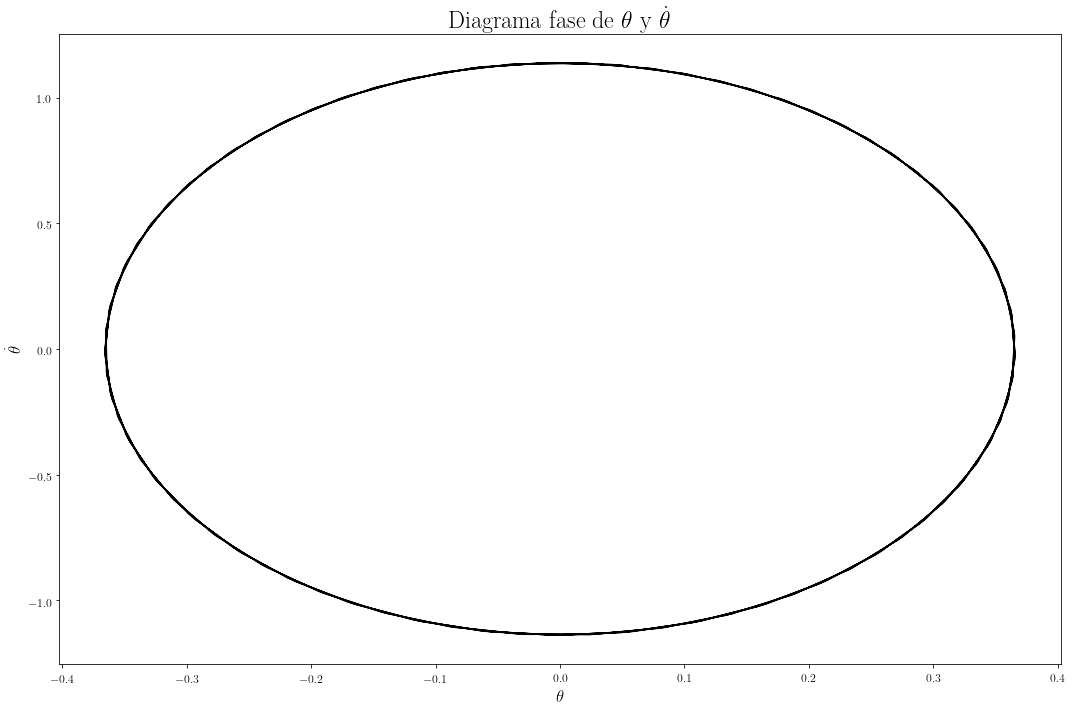
\includegraphics[scale=0.2]{img/sp_phase_diagram_theta_dtheta.png}
 % sp_plot_theta_theta_linear.png: 1072x712 px, 72dpi, 37.83x25.12 cm, bb=0 0 1072 712
 \caption{Diagrama de fase $\theta$ y $\dot{\theta}$ sin fricción.}
 \label{fig: phase theta dtheta}
\end{figure}

\begin{figure}[h]
 \centering
 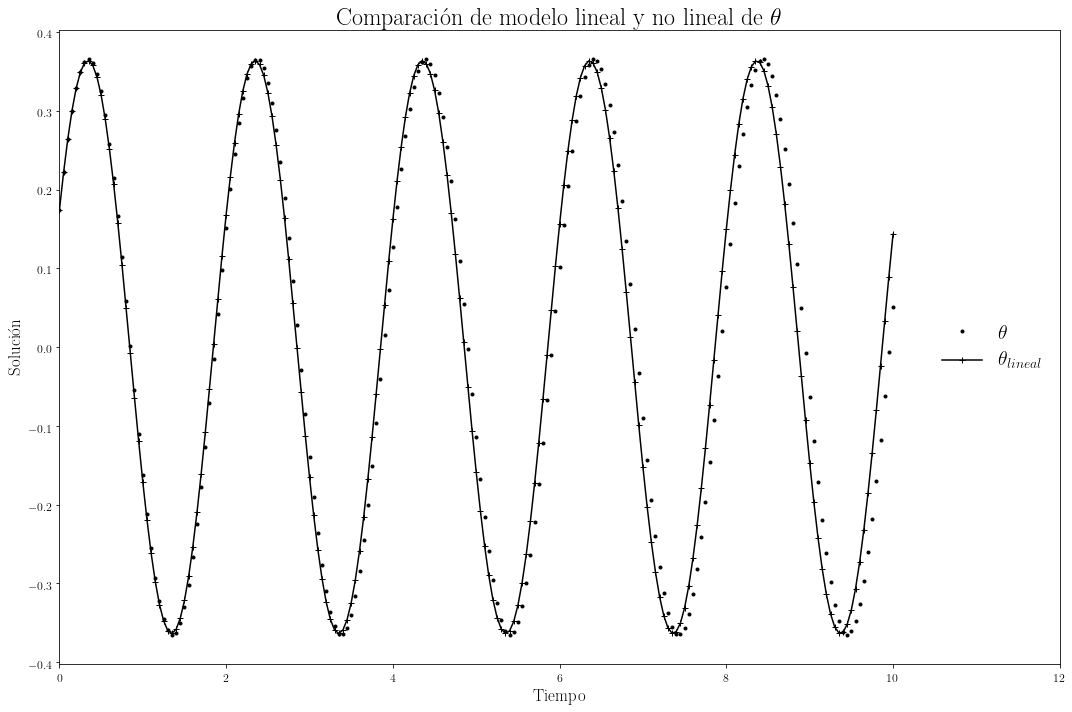
\includegraphics[scale=0.2]{img/sp_plot_theta_theta_linear.png}
 % sp_plot_theta_theta_linear.png: 1072x712 px, 72dpi, 37.83x25.12 cm, bb=0 0 1072 712
 \caption{Comportamiento de $\theta$ sin fricción.}
 \label{fig: theta}
\end{figure}

\begin{figure}[h]
 \centering
 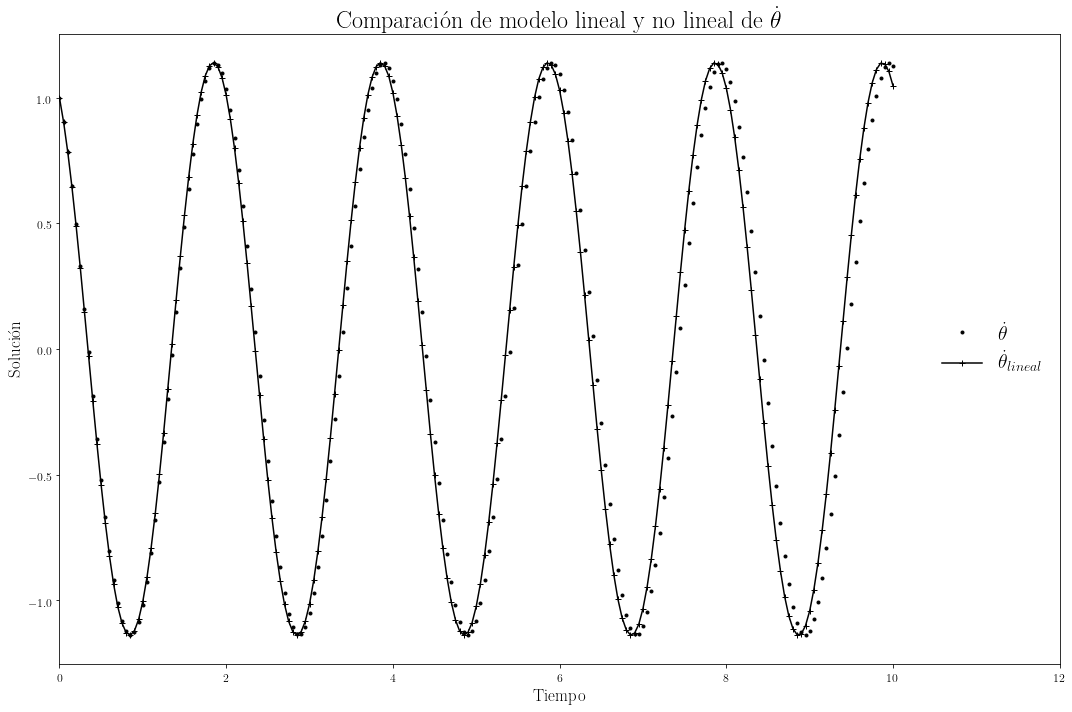
\includegraphics[scale=0.2]{img/sp_plot_dtheta_dtheta_linear.png}
 % sp_plot_theta_theta_linear.png: 1072x712 px, 72dpi, 37.83x25.12 cm, bb=0 0 1072 712
 \caption{Comportamiento de $\dot{\theta}$ sin fricción.}
 \label{fig: dtheta}
\end{figure}

\pagebreak

\subsection*{Caso con fricción}

Al introducir fricción al sistema, se observa en el diagrama 
de fase (\ref{fig: phase theta dtheta friction}) que el 
sistema converge a un estado de equilibrio en $\theta$ igual 
a cero. A su vez, las gráficas de posición angular (figura 
\ref{fig: theta friction}) y velocidad angular (figura 
\ref{fig: dtheta friction}) tienden a un punto de equlibrio 
en cero conforme el tiempo avanza.

\begin{figure}[h]
 \centering
 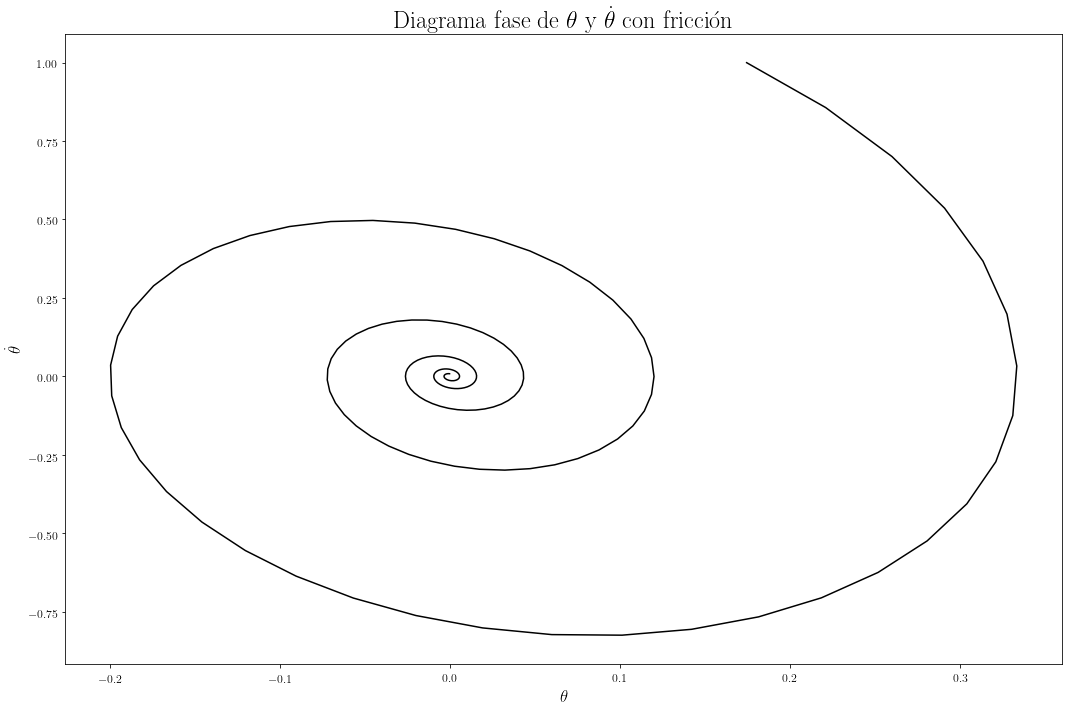
\includegraphics[scale=0.2]{img/sp_phase_diagram_theta_dtheta_friction.png}
 % sp_plot_theta_theta_linear.png: 1072x712 px, 72dpi, 37.83x25.12 cm, bb=0 0 1072 712
 \caption{Diagrama de fase $\theta$ y $\dot{\theta}$ con fricción.}
 \label{fig: phase theta dtheta friction}
\end{figure}

\begin{figure}
 \centering
 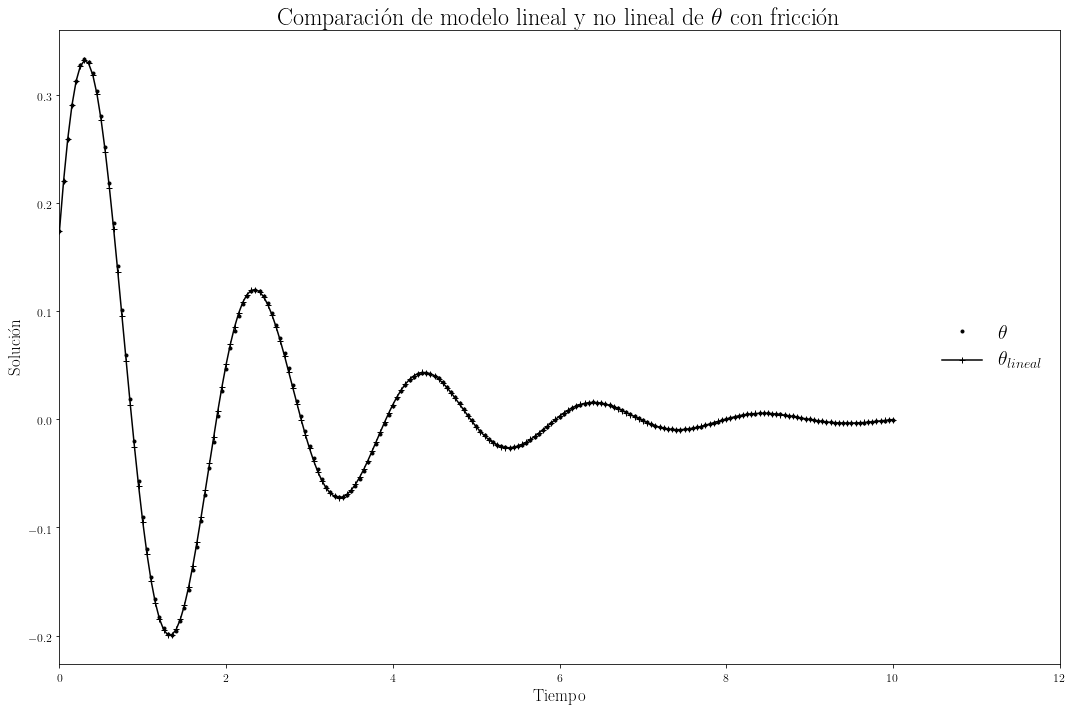
\includegraphics[scale=0.2]{img/sp_plot_theta_theta_linear_friction.png}
 % sp_plot_theta_theta_linear.png: 1072x712 px, 72dpi, 37.83x25.12 cm, bb=0 0 1072 712
 \caption{Comportamiento de $\theta$ con fricción.}
 \label{fig: theta friction}
\end{figure}

\begin{figure}
 \centering
 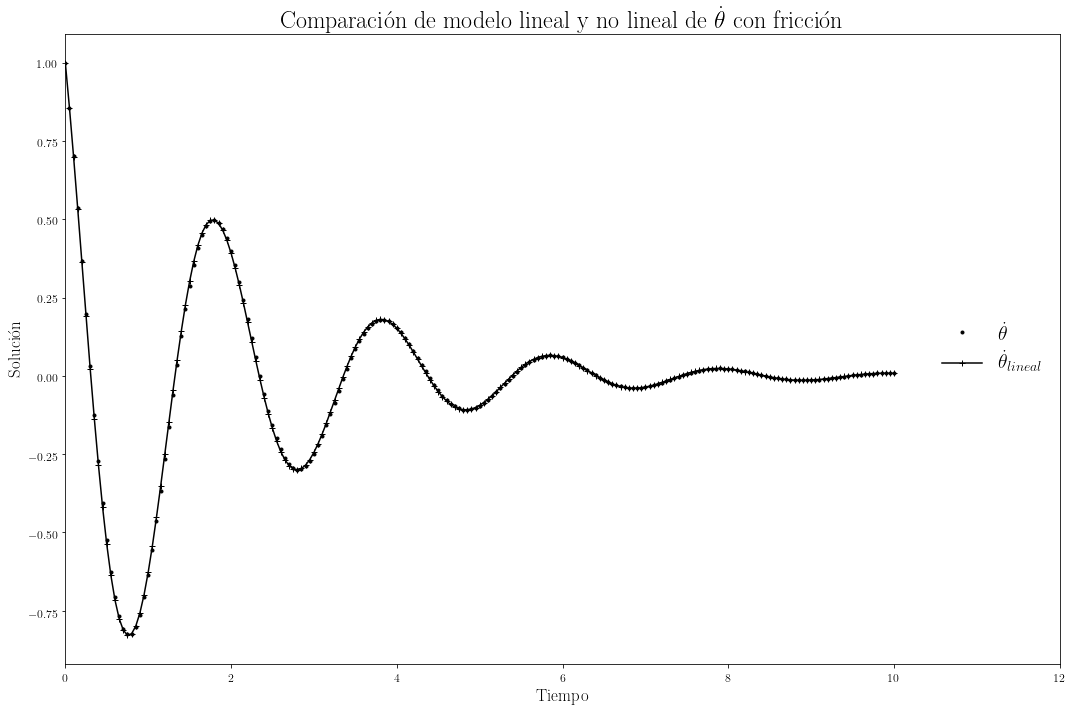
\includegraphics[scale=0.2]{img/sp_plot_dtheta_dtheta_linear_friction.png}
 % sp_plot_theta_theta_linear.png: 1072x712 px, 72dpi, 37.83x25.12 cm, bb=0 0 1072 712
 \caption{Comportamiento de $\dot{\theta}$ con fricción.}
 \label{fig: dtheta friction}
\end{figure}

% \printbibliography



\pagebreak

\section*{Péndulo Doble}

Se evaluó la simulación de péndulo doble para las condiciones mostradas en la table \ref{table: dp initial conditions}. Se emplearon dos modelos para la simulación: 
modelo con gravedad (energía potencial) y sin gravedad.


\begin{table}[h]
\begin{center}
\centering
\begin{tabular}{cccc}
\hline
Tiempo inicial ($t_0$) & 0  & Posición angular inicial ($\theta_0$) & $\frac{\pi}{4}$ \\
%\hline
Tiempo final ($t_f$) & 10 & Velocidad angular inicial ($\dot{\theta}_0$)& $1$\\
Masa ($m$) & 1 &  Posición angular inicial ($\alpha_0$) & $0$\\
Longitud ($l$) & 1 & Velocidad angular inicial ($\dot{\alpha}_0$)& $0$\\
Constante de gravedad ($g$) & $9.81$ &  & \\
\hline
\end{tabular}
\end{center}
 \caption{Condiciones de simulación.}
 \label{table: dp initial conditions}
\end{table}

\pagebreak

Se observa en la figura \ref{fig: dp theta thetaG} que el valor de $\theta$ incrementa de manera lineal en función de la velocidad angular inicial si no hay gravedad presente en el sistema. 
El comportamiento para el caso de gravedad presente en el sistema es más complejo debido al efecto que $\alpha$ tiene sobre $\theta$.



\begin{figure}[h!]
 \centering
 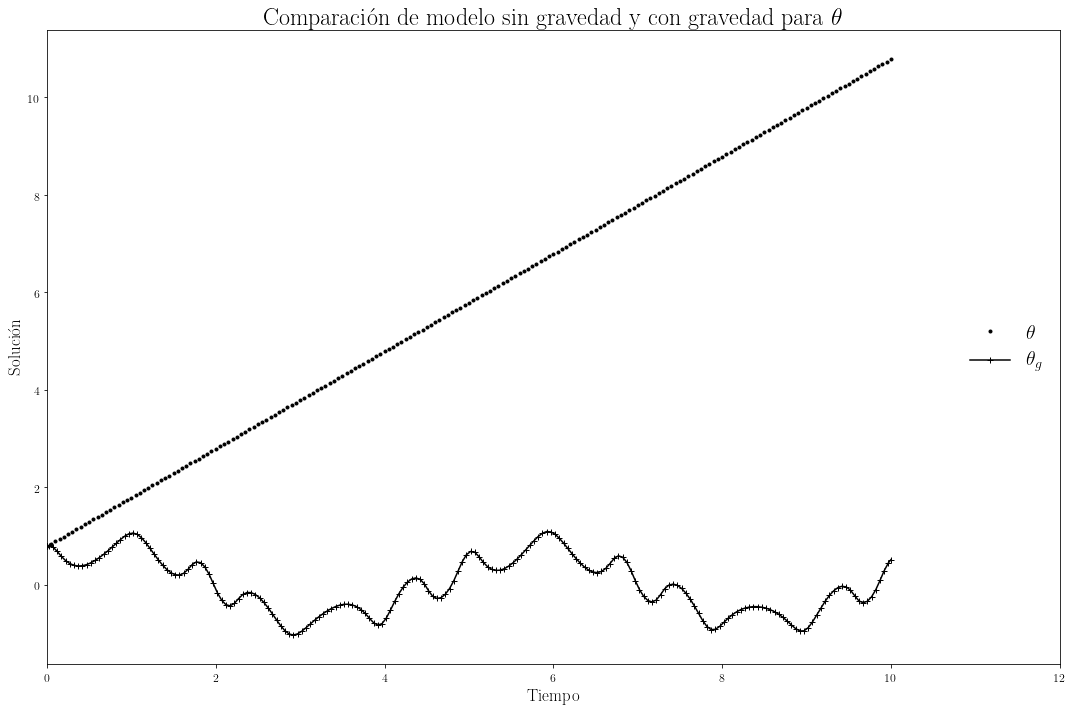
\includegraphics[scale=0.2]{img/dp_theta_thetaG.png}
 \caption{Comportamiento de $\theta$ sin gravedad y con gravedad.}
 \label{fig: dp theta thetaG}
\end{figure}

\pagebreak



El segundo objeto en el sistema, con posición angular $\alpha$ se muestra en la figura \ref{fig: dp alpha alphaG}.
Para el caso sin gravedad, $\alpha$ no experimenta cambio alguno, y su comportamiento es errático al introducir
gravedad en el sistema.

\begin{figure}[h]
 \centering
 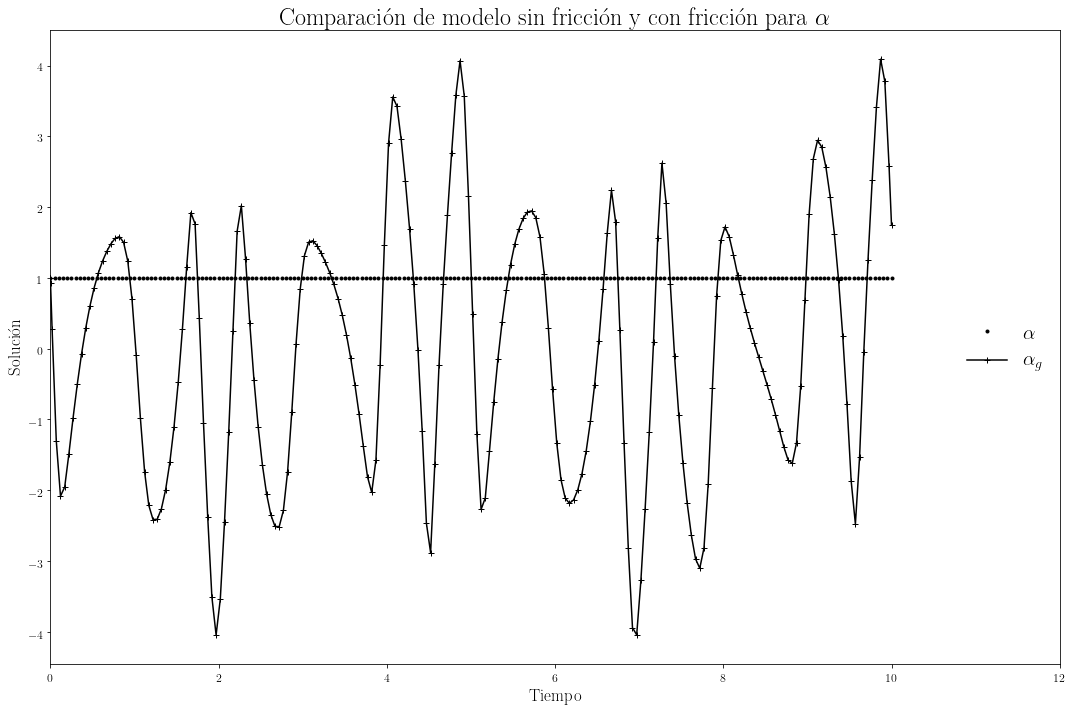
\includegraphics[scale=0.2]{img/dp_alpha_alphaG.png}
 \caption{Comportamiento de $\alpha$ sin gravedad y con gravedad.}
 \label{fig: dp alpha alphaG}
\end{figure}

\pagebreak

Las figuras \ref{fig: dp phase theta dtheta}, \ref{fig: dp phase theta dtheta G}, \ref{fig: dp phase alpha dalpha} y \ref{fig: dp phase alpha dalpha G} muestran los diagramas fase del sistema.

\begin{figure}[h]
 \centering
 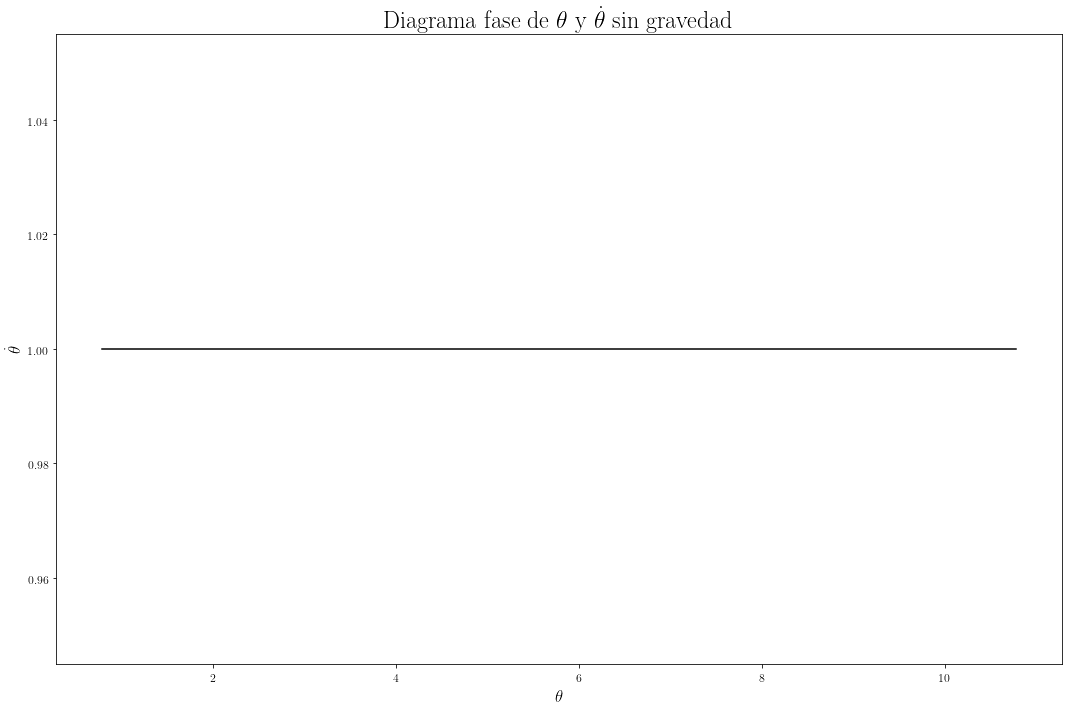
\includegraphics[scale=0.2]{img/dp_phase_theta_dtheta.png}
 \caption{Diagrama de fase para $\theta$ y $\dot{\theta}$ sin gravedad.}
 \label{fig: dp phase theta dtheta}
\end{figure}

\begin{figure}[h]
 \centering
 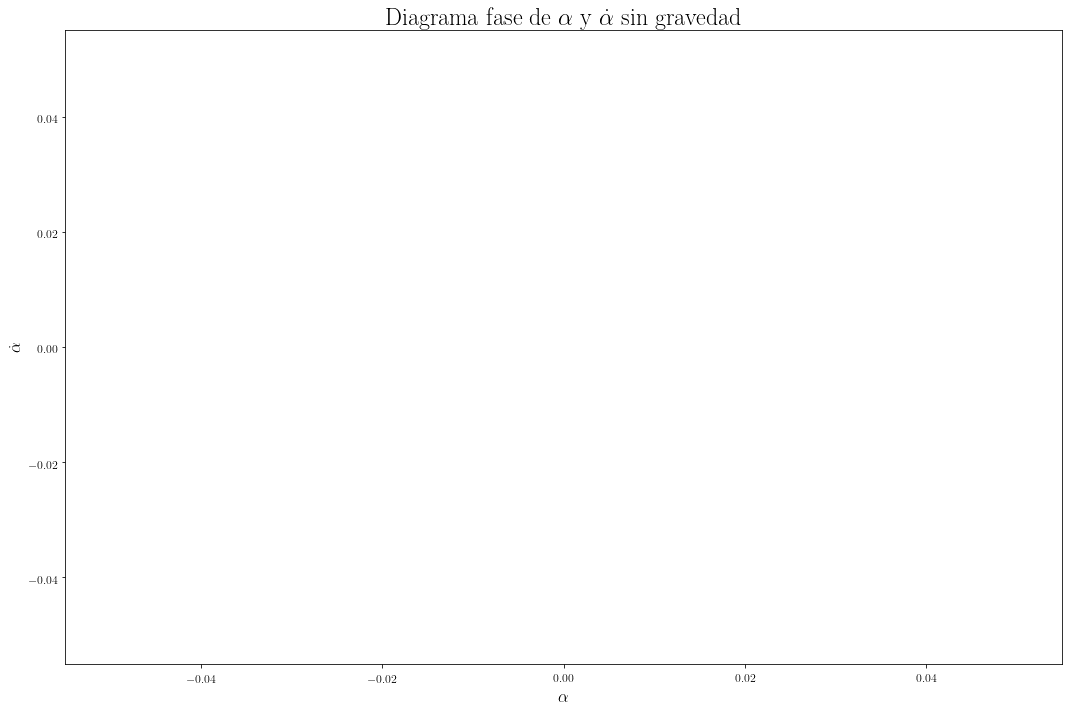
\includegraphics[scale=0.2]{img/dp_phase_alpha_dalpha.png}
 \caption{Diagrama de fase para $\alpha$ y $\dot{\alpha}$ sin gravedad.}
 \label{fig: dp phase alpha dalpha}
\end{figure}

\begin{figure}[h]
 \centering
 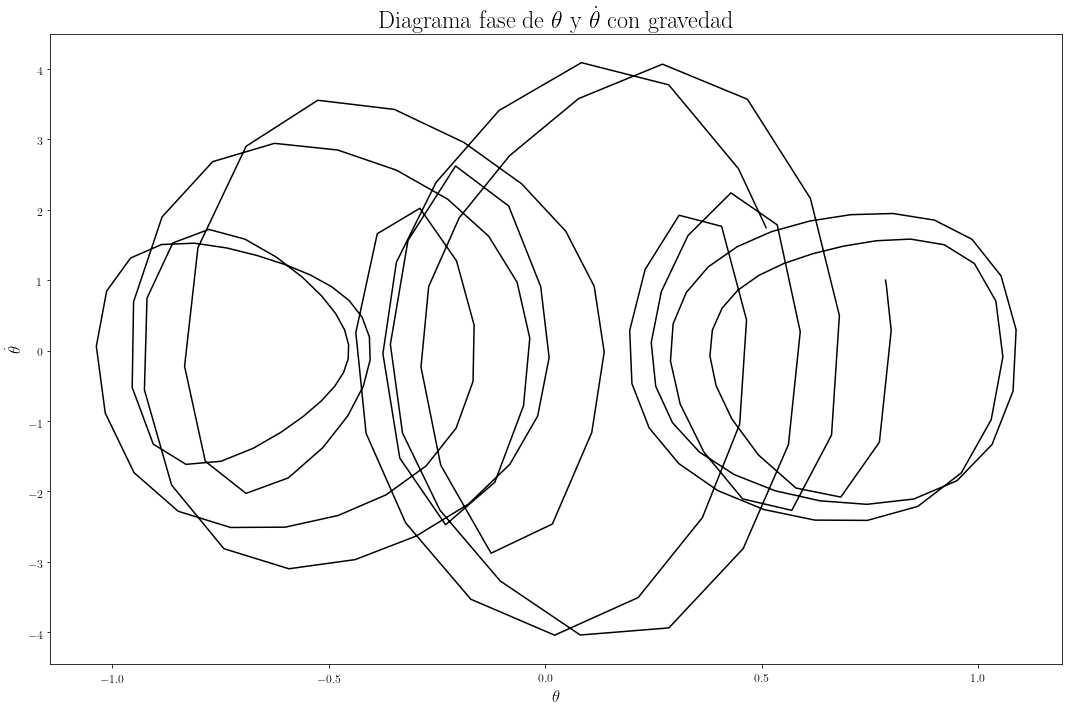
\includegraphics[scale=0.2]{img/dp_phase_theta_dtheta_G.png}
 \caption{Diagrama de fase para $\theta$ y $\dot{\theta}$ con gravedad.}
 \label{fig: dp phase theta dtheta G}
\end{figure}

\begin{figure}[h]
 \centering
 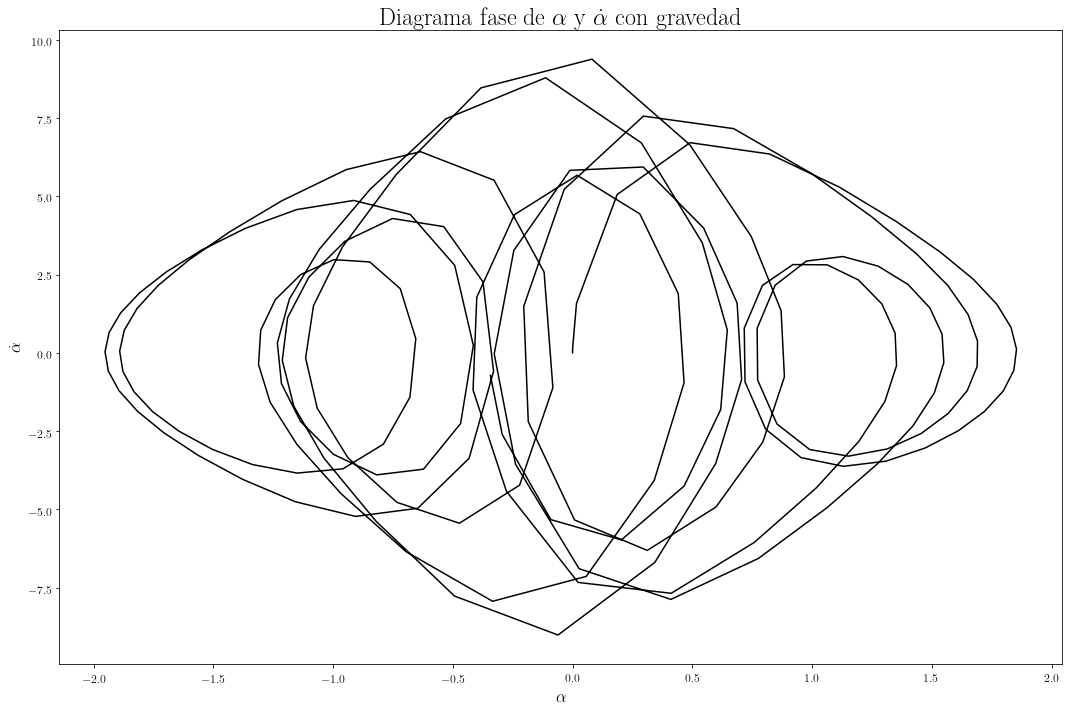
\includegraphics[scale=0.2]{img/dp_phase_alpha_dalpha_G.png}
 \caption{Diagrama de fase para $\alpha$ y $\dot{\alpha}$ con gravedad.}
 \label{fig: dp phase alpha dalpha G}
\end{figure}



\pagebreak

\section*{Péndulo Invertido}

La simulación de péndulo invertido comparó los siguientes dos modelos:

\begin{itemize}
 \item Modelo referencia
\begin{equation*}
  \begin{pmatrix}
  m_c + m_p & l m_p \cos (\theta) \\
  m_p l \cos (\theta) & m_p l^2\\
 \end{pmatrix}
 \begin{pmatrix}
  \ddot{x} \\
  \ddot{\theta}
 \end{pmatrix}
 +
 \begin{pmatrix}
  -\dot{\theta}^2 l m_p \sin(\theta) \\
  m_p l g \sin(\theta)
 \end{pmatrix}
 = 
 \begin{pmatrix}
  F \\
  0
 \end{pmatrix}
\end{equation*}


 \item Modelo Miriam
\begin{equation*}
  \begin{pmatrix}
  m_c + m_p & l m_p \cos (\theta) \\
  m_p l \cos (\theta) & m_p l^2\\
 \end{pmatrix}
 \begin{pmatrix}
  \ddot{x} \\
  \ddot{\theta}
 \end{pmatrix}
 +
 \begin{pmatrix}
  -\dot{\theta}^2 l m_p \sin(\theta) \\
  m_p l g \sin(\theta) + 2 l m_p \dot{x} \dot{\theta} \sin(\theta)
 \end{pmatrix}
 = 
 \begin{pmatrix}
  F \\
  0
 \end{pmatrix}
\end{equation*}
\end{itemize}

La tabla \ref{table: ip initial conditions} presenta las condiciones de la simulación.

\begin{table}[h]
\begin{center}
\centering
\begin{tabular}{cccc}
\hline
Tiempo inicial ($t_0$) & 0  & Posición inicial ($x_0$) & $0$ \\
%\hline
Tiempo final ($t_f$) & 10 & Velocidad inicial ($\dot{x}_0$)& $0$\\
Masa del vehículo ($m_c$) & 1 &  Posición angular inicial ($\theta_0$) & $\dfrac{3 \pi}{4}$\\
Masa del péndulo ($m_p$) & 1 & Velocidad angular inicial ($\dot{\theta}_0$)& $0$\\
Constante de gravedad ($g$) & $9.81$ & Longitud ($l$) & $1$ \\
Modelo de fuerza ($F$) & $0$ & & \\
\hline
\end{tabular}
\end{center}
 \caption{Condiciones de simulación.}
 \label{table: ip initial conditions}
\end{table}

Se observa que para las mismas condiciones iniciales, el segundo modelo presenta un desfase en el período en la posición $x$ (figura \ref{fig: ip x}) y la posición angular $\theta$ (figura \ref{fig: ip theta}) casi inmediatamente.

\begin{figure}[h]
 \centering
 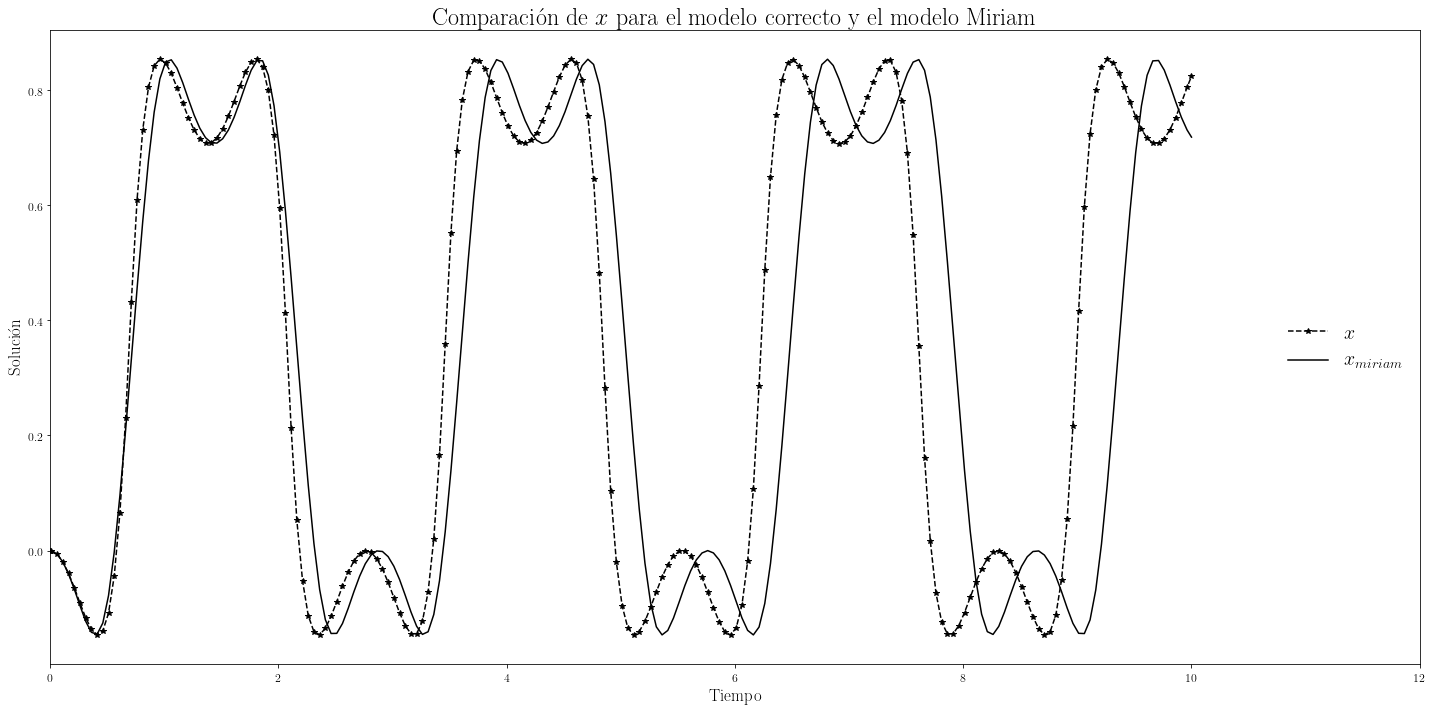
\includegraphics[scale=0.2]{img/ip_x.png}
 % ip_theta.png: 1432x712 px, 72dpi, 50.53x25.12 cm, bb=0 0 1432 712
 \caption{Comportamiento de $x$ para los modelos de péndulo invertido.}
 \label{fig: ip x}
\end{figure}

\begin{figure}[h]
 \centering
 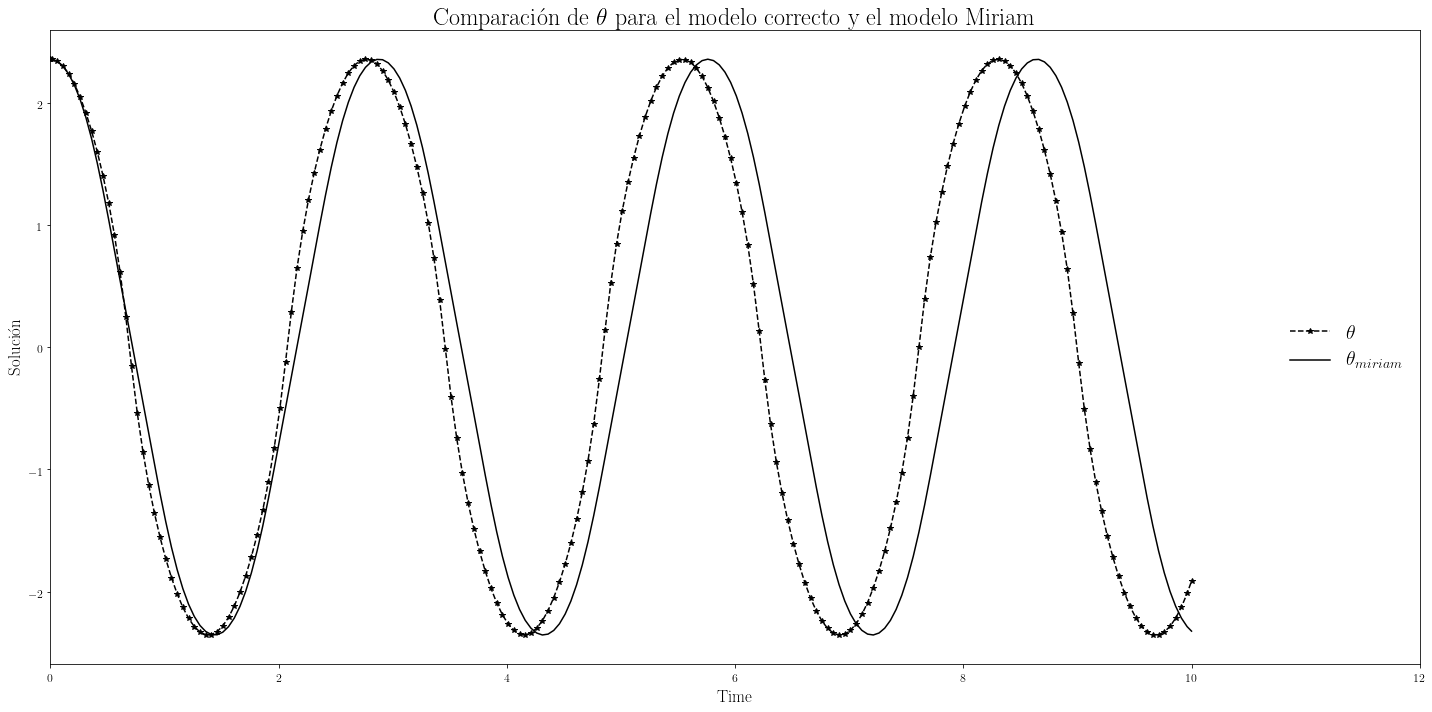
\includegraphics[scale=0.2]{img/ip_theta.png}
 % ip_theta.png: 1432x712 px, 72dpi, 50.53x25.12 cm, bb=0 0 1432 712
 \caption{Comportamiento de $\theta$ para los modelos de péndulo invertido.}
 \label{fig: ip theta}
\end{figure}



\end{document}
